\documentclass[12pt]{report}
\usepackage[utf8]{inputenc}
\usepackage[russian]{babel}
%\usepackage[14pt]{extsizes}
\usepackage{listings}

% Для листинга кода:
\lstset{ %
language=python,                 % выбор языка для подсветки (здесь это С)
basicstyle=\small\sffamily, % размер и начертание шрифта для подсветки кода
numbers=left,               % где поставить нумерацию строк (слева\справа)
numberstyle=\tiny,           % размер шрифта для номеров строк
stepnumber=1,                   % размер шага между двумя номерами строк
numbersep=5pt,                % как далеко отстоят номера строк от подсвечиваемого кода
showspaces=false,            % показывать или нет пробелы специальными отступами
showstringspaces=false,      % показывать или нет пробелы в строках
showtabs=false,             % показывать или нет табуляцию в строках
frame=single,              % рисовать рамку вокруг кода
tabsize=2,                 % размер табуляции по умолчанию равен 2 пробелам
captionpos=t,              % позиция заголовка вверху [t] или внизу [b] 
breaklines=true,           % автоматически переносить строки (да\нет)
breakatwhitespace=false, % переносить строки только если есть пробел
escapeinside={\#*}{*)}   % если нужно добавить комментарии в коде
}

% Для измененных титулов глав:
\usepackage{titlesec, blindtext, color} % подключаем нужные пакеты
\definecolor{gray75}{gray}{0.75} % определяем цвет
\newcommand{\hsp}{\hspace{20pt}} % длина линии в 20pt
% titleformat определяет стиль
\titleformat{\chapter}[hang]{\Huge\bfseries}{\thechapter\hsp\textcolor{gray75}{|}\hsp}{0pt}{\Huge\bfseries}


% plot
\usepackage{pgfplots}
\usepackage{filecontents}
\usetikzlibrary{datavisualization}
\usetikzlibrary{datavisualization.formats.functions}

\begin{document}
 
%\def\chaptername{} % убирает "Глава"
\begin{titlepage}
	\centering
	{\scshape\LARGE МГТУ им. Баумана \par}
	\vspace{3cm}
	{\scshape\Large Лабораторная работа №4\par}
	\vspace{0.5cm}	
	{\scshape\Large По курсу: "Анализ алгоритмов"\par}
	\vspace{1.5cm}
	{\huge\bfseries Параллельное программирование\par}
	\vspace{2cm}
	\Large Работу выполнил: студент группы ИУ7-53Б Наместник Анастасия\par
	\vspace{0.5cm}
	\LargeПреподаватели:  Волкова Л.Л., Строганов Ю.В.\par

	\vfill
	\large \textit {Москва, 2020} \par
\end{titlepage}

\tableofcontents

\newpage
\chapter*{Введение}
\addcontentsline{toc}{chapter}{Введение}

	\textbf{Параллельное программирование} служит для создания программ, эффективно использующих вычислительные ресурсы за счет одновременного исполнения кода на нескольких вычислительных узлах. Использование параллельного программирования становится наиболее необходимым, поскольку позволяет максимально эффективно использовать возможности многоядерных процессоров и многопроцессорных систем. По ряду причин, включая повышение потребления энергии и ограничения пропускной способности памяти, увеличивать тактовую частоту современных процессоров стало невозможно. Вместо этого производители процессоров стали увеличивать их производительность за счет размещения в одном чипе нескольких вычислительных ядер, не меняя или даже снижая тактовую частоту. Поэтому для увеличения скорости работы приложений теперь следует по-новому подходить к организации кода, а именно - оптимизировать программы под многоядерные системы \cite{MicrosoftPar}.
 В рамках этой лабораторной работы будет рассмотрено параллельное программирование на примере стандартного алгоритма умножения матриц.

	Целью данной лабораторной работы является изучение и реализация параллельного программирования для решения задачи умножения матриц, а также сравнительный анализ затрачиваемых временных ресурсов при параллельной и однопоточной реализаций одного и того же алгоритма.

В данной лабораторной работе требуется решить четыре задачи.
\begin{enumerate}
\item Изучить основы многопоточного программирования.
\item  Придумать два варианта многопоточной реализации стандартного алгоритма умножения матриц.
\item Программно реализовать стандартный алгоритм умножения матриц в однопоточном режиме.
\item Сделать сравнительный анализ по затрачиваемым ресурсам (времени) компьютера на реализацию каждого рассмотренного алгоритма.
\end{enumerate}


\chapter{Аналитическая часть}
 
 В данной лабораторной работе метод параллельного программирования будет применен к стандартному алгоритму умножения матриц. Ниже будут представлены теоретические сведения, необходимые для программной реализации этой задачи.
 
 \section{Стандартный алгоритм умножения матриц}
 
 Допустим, имеются матрицы A (формула \ref{eq:ref1}) и B (формула \ref{eq:ref2}).
 
 \begin{equation}
	A = \left(
	\begin{array}{cccc}
			a_{11} & a_{12} & \ldots & a_{1m} \\
			a_{21} & a_{22} & \ldots & a_{2m} \\
			\vdots & \vdots & \ddots & \vdots \\
			a_{n1} & a_{n2} & \ldots & a_{nm}
		\end{array}
	\right)
	\label{eq:ref1}
\end{equation}

\begin{equation}
	B = \left(
	\begin{array}{cccc}
			b_{11} & b_{12} & \ldots & b_{1m} \\
			b_{21} & b_{22} & \ldots & b_{2m} \\
			\vdots & \vdots & \ddots & \vdots \\
			b_{n1} & b_{n2} & \ldots & b_{nm}
		\end{array}
	\right)
	\label{eq:ref2}
\end{equation}

Матрица C = AB будет размерностью $l \times n$, 
где матрица A размерностью $l \times m$, а матрица B $m \times n$
Тогда каждый элемент матрицы C выражается формулой (\ref{eq:ref3})

\begin{equation}
	\begin{array}{cc}
		c_{ij} = \sum\limits_{r=1}^m a_{ir}b_{ri} & (i=1,2,\dots l; j=1,2,\dots n)
	\end{array}
	\label{eq:ref3}
\end{equation}

Процесс произведения матриц проиллюстрирован рисунком 1.1.

\begin{center}
		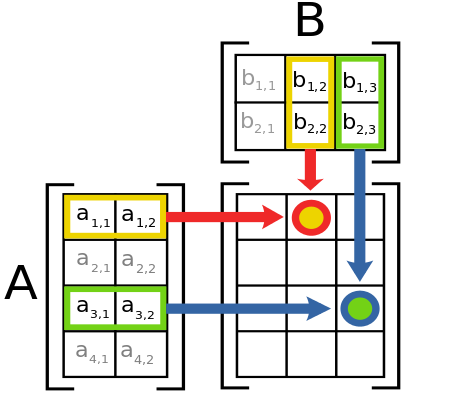
\includegraphics[scale=0.6]{pics/matrix_mult.png}
		
			Рис 1.1: Произведение матриц
\end{center}

Важно отметить низкое быстродействие данного алгоритма и достаточно высокую трудоемкость (≈ 13NMQ). Следовательно, распараллеливание стандартного алгоритма умножения матриц должно повысить эффективность алгоритма.

\section{Параллельное программирование}

Параллельное программирование - это техника программирования, которая использует преимущества многоядерных или многопроцессорных компьютеров и является подмножеством более широкого понятия многопоточности. Таким образом, Параллельные вычисления - способ организации компьютерных вычислений, при котором программы разрабатываются, как набор взаимодействующих вычислительных процессов, работающих асинхронно и при этом одновременно \cite{MicrosoftPar}.

\section{Параллельная реализация стандартного алгоритма умножения матриц}

Ввиду того, что в стандартном алгоритме умножения матриц каждая строка и столбец результирующей матрицы считаются независимо, можно выделить два варианта применения многопоточного программирования к данному алгоритму.
\begin{enumerate}
\item Распараллеливание по строкам (строки результирующей матрицы вычисляются параллельно).
\item  Распараллеливание по столбцам (столбцы результирующей матрицы вычисляются параллельно).
\end{enumerate}

\section{Вывод}

В данном разделе были рассмотрены теоретические сведения о стандартном алгоритме умножения матриц и параллельном программировании, а также были приведены два варианта применения этого подхода к описанному выше алгоритму.
 
\chapter{Конструкторская часть}

В данном разделе будут представлены схемы последовательной и параллельной реализаций стандартного алгоритма умножения матриц.

\section{Стандартный алгоритм произведения матриц}

На рисунке 2.2 представлена схема стандартного алгоритма произведения матриц.

\begin{center}
		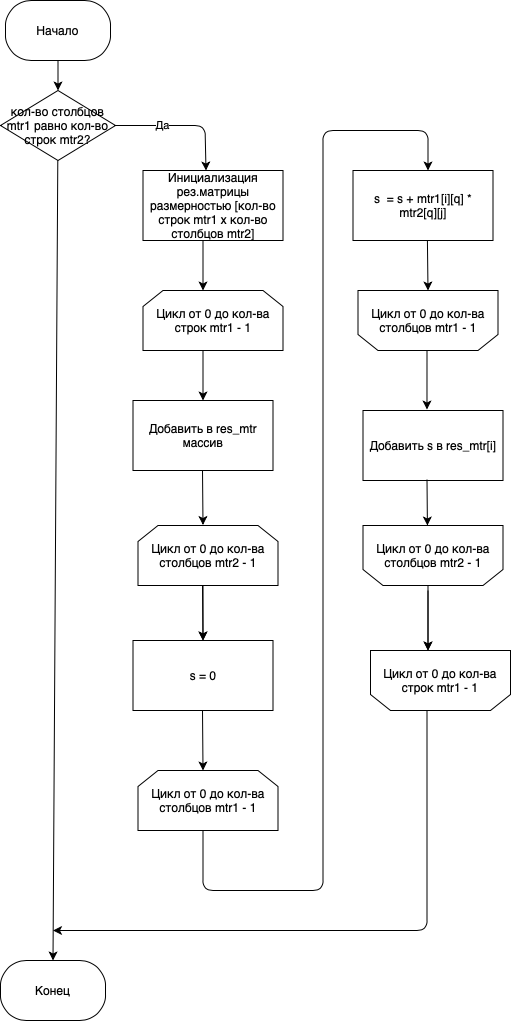
\includegraphics[scale=0.6]{schema/StandMtr.png}
		
			Рис 2.1: Схема стандартного алгоритма произведения матриц
\end{center}

\newpage
\section{Параллельная реализация при обходе по строкам}

На рисунке 2.3 представлена схема главного потока параллельной реализации стандартного алгоритма произведения матриц.

\begin{center}
		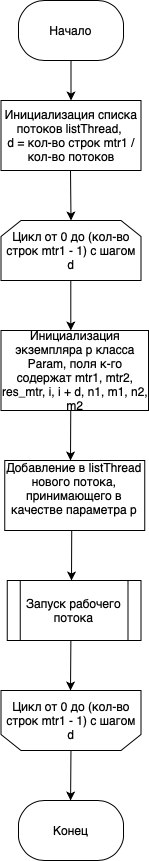
\includegraphics[scale=0.5]{schema/ParRowMain.png}
		
			Рис 2.3: Схема главного потока (обход по строкам)
\end{center}

На рисунке 2.4 представлена схема рабочего потока параллельной реализации стандартного алгоритма произведения матриц.

\begin{center}
		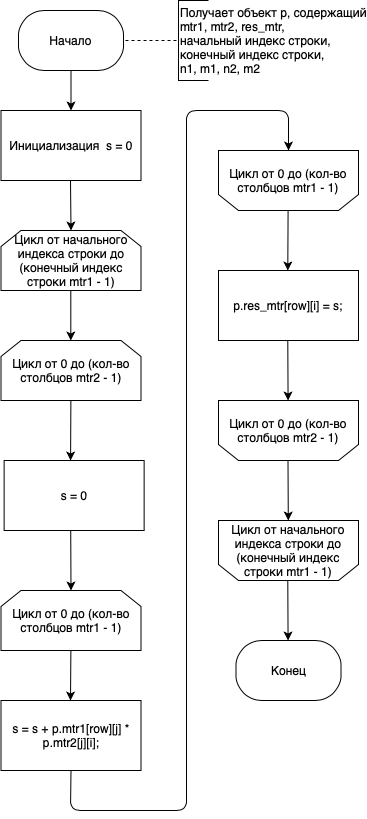
\includegraphics[scale=0.6]{schema/ParRowWork.png}
		
			Рис 2.4: Схема рабочего потока (обход по строкам)
\end{center}

\newpage
\section{Параллельная реализация при обходе по столбцам}

На рисунке 2.5 представлена схема главного потока параллельной реализации стандартного алгоритма произведения матриц.

\begin{center}
		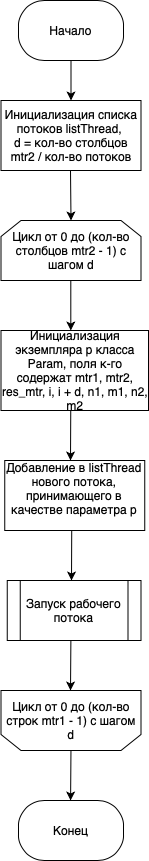
\includegraphics[scale=0.5]{schema/ParColMain.png}
		
			Рис 2.5: Схема главного потока (обход по столбцам)
\end{center}

На рисунке 2.6 представлена схема рабочего потока параллельной реализации стандартного алгоритма произведения матриц.

\begin{center}
		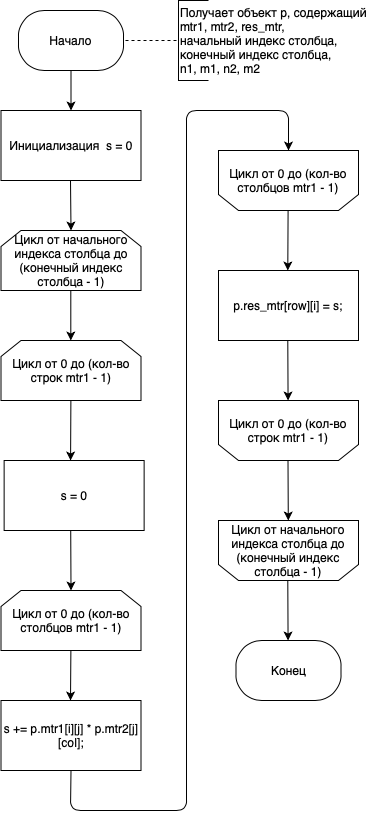
\includegraphics[scale=0.6]{schema/ParColWork.png}
		
			Рис 2.6: Схема рабочего потока (обход по столбцам)
\end{center}
\section{Вывод}
В данном разделе были рассмотрены 5 схем: стандартного алгоритма умножения матриц, главного и рабочего потоков параллельной реализации этого алгоритма при обходе по строкам, главного и рабочего потоков параллельной реализации этого алгоритма при обходе по столбцам. 

\chapter{Технологическая часть}
\section{Выбор языка программирования}
В данной лабораторной работе использовался язык программирования - С\# \cite{C}, так как данный язык программирования поддерживает параллельное программирования, он является нативным. В качестве интегрированной среды разработки использовалась Visual studio  \cite{Vs}. Для замеров времени использовались методы Start() и Stop() класса Stopwatch \cite{Stopwatch}.  Для генерации матрицы использовался метод Next класса Random \cite{Rand}.

\section{Сведения о модулях программы}
Программа состоит из следующих модулей.
\begin{itemize}
	\item Program.cs - однопоточная реализация.
	\item ParallelMult.cs - многопоточная реализация.
\end{itemize}

На листинге 3.1 представлена подпрограмма однопоточной реализации стандартного алгоритма умножения матриц
\begin{lstlisting}[label=some-code,caption=Подпрограмма однопоточной реализации стандартного алгоритма умножения матриц]
public static int[][] StandMult(int[][] mtr1, int[][] mtr2)
        {
            int n1 = mtr1.Length;
            int n2 = mtr2.Length;

            if (n1 == 0 || n2 == 0)
                return null;

            int m1 = mtr1[0].Length;
            int m2 = mtr2[0].Length;

            if (m1 != n2)
                return null;

            int[][] res\_mtr = new int[n1][];
            for (int i = 0; i < n1; i++)
                res\_mtr[i] = new int[m2];

            for (int i = 0; i < n1; i++)
            {
                for (int j = 0; j < m2; j++)
                {
                    for (int q = 0; q < m1; q++)
                    {
                        res\_mtr[i][j] = res\_mtr[i][j] + mtr1[i][q] * mtr2[q][j];
                    }
                }
            }

            return res\_mtr;
        }\end{lstlisting}

На листинге 3.2 представлена подпрограмма главного потока многопоточной реализации стандартного алгоритма умножения матриц при обходе по строкам.

\begin{lstlisting}[label=some-code,caption=Подпрограмма главного потока многопоточной реализации стандартного алгоритма умножения матриц (обход по строкам)]
public static void ParallelMultFirst(int[][] res_mtr, int[][] mtr1, int[][] mtr2, int n1, int m1, int n2, int m2, int tc)
        {
            List<Thread> listThread = new List<Thread>();
            int d = n1 / tc;
            int j = 0;
            
            for (int i = 0; i < n1; i += d)
            {
                //Console.WriteLine("Main thread:");
                Param p = new Param(res\_mtr, mtr1, mtr2, i, i + d, n1, m1, n2, m2);
                 
                listThread.Add(new Thread(new ParameterizedThreadStart(ParallelMultRow)));
                listThread[j].Start(p); 
                j += 1;
             }
     
            foreach (var elem in listThread)
            {

                if (elem.IsAlive)
                    elem.Join();
            }
        }
\end{lstlisting}

На листинге 3.3 представлена подпрограмма рабочего потока многопоточной реализации стандартного алгоритма умножения матриц при обходе по строкам.

\begin{lstlisting}[label=some-code,caption=Подпрограмма рабочего потока многопоточной реализации стандартного алгоритма умножения матриц (обход по строкам)]
public static void ParallelMultRow(object obj)
        {
            Param p = (Param)obj;
            int s = 0;

            for (int row = p.start; row < p.end; row++)
            {
                for (int i = 0; i < p.m2; i++)
                {
                    s = 0;
                    for (int j = 0; j < p.m1; j++)
                    {
                        s += p.mtr1[row][j] * p.mtr2[j][i];
                    }
                    p.res\_mtr[row][i] = s;
                }
            }
        }
\end{lstlisting}

На листинге 3.4 представлена подпрограмма главного потока многопоточной реализации стандартного алгоритма умножения матриц при обходе по столбцам.

\begin{lstlisting}[label=some-code,caption= Подпрограмма главного потока многопоточной реализации стандартного алгоритма умножения матриц (обход по столбцам)]
public static void ParallelMultSecond(int[][] res_mtr, int[][] mtr1, int[][] mtr2, int n1, int m1, int n2, int m2, int tc)
        {
            int d = m2 / tc;
            int j = 0;

            List<Thread> listThread = new List<Thread>();

            for (int i = 0; i < m2; i += d)
            {
                Param p = new Param(res\_mtr, mtr1, mtr2, i, i + d, n1, m1, n2, m2);
                
                listThread.Add(new Thread(new ParameterizedThreadStart(ParallelMultCol)));
                listThread[j].Start(p); 
                j += 1;
            }
            //Console.WriteLine("Main thread:");

            foreach (var elem in listThread)
            {
                if (elem.IsAlive)
                    elem.Join();
            }
        }
\end{lstlisting}

На листинге 3.5 представлена подпрограмма рабочего потока многопоточной реализации стандартного алгоритма умножения матриц при обходе по столбцам.

\begin{lstlisting}[label=some-code,caption= Подпрограмма рабочего потока многопоточной реализации стандартного алгоритма умножения матриц (обход по столбцам)]
public static void ParallelMultCol(object obj)
        {
            Param p = (Param)obj;
            int s = 0;

            for (int col = p.start; col < p.end; col++)
            {
                for (int i = 0; i < p.n1; i++)
                {
                    s = 0;
                    for (int j = 0; j < p.m1; j++)
                    {
                        s += p.mtr1[i][j] * p.mtr2[j][col];
                    }
                    p.res\_mtr[i][col] = s;
                }
            }
        }
 \end{lstlisting}

На листинге 3.6 представлена подпрограмма создания матрицы.

\begin{lstlisting}[label=some-code,caption=Подпрограмма создания матрицы]
public static int[][] InitMatrix(int n, int m)
        {
            int[][] mtr = new int[n][];
            for (int i = 0; i < n; i++)
                mtr[i] = new int[m];

            Console.WriteLine("Enter the matrix: ");
            for (int i = 0; i < n; i++)
            {
                for (int j = 0; j < m; j++)
                {
                    mtr[i][j] = Convert.ToInt32(Console.ReadLine());
                }
            }
            retu

\end{lstlisting}

На листинге 3.7 представлена подпрограмма рандомной генерации матрицы .

\begin{lstlisting}[label=some-code,caption=Подпрограмма создания матрицы с использованием метода Next класса Random \cite{Rand}]
public static int[][] RandomMatrix(int n, int m)
        {
            int[][] mtr = new int[n][];
            for (int i = 0; i < n; i++)
                mtr[i] = new int[m];
          
            for (int i = 0; i < n; i++)
            {
                for (int j = 0; j < m; j++)
                {
                    mtr[i][j] = rand.Next(1, 10);
                }
            }
            return mtr;
        }
\end{lstlisting}

\begin{lstlisting}[label=some-code,caption=класс Param]
class Param
    {
        public int[][] res\_mtr, mtr1, mtr2;
        public int n1, m1, n2, m2;
        public int start, end;

        public Param(int[][] res\_mtr, int[][] mtr1, int[][] mtr2, int start, int end, int n1, int m1, int n2, int m2)
        {
            this.res\_mtr = res\_mtr;
            this.mtr1 = mtr1;
            this.mtr2 = mtr2;
            this.n1 = n1;
            this.m1 = m1;
            this.n2 = n2;
            this.m2 = m2;
            this.start = start;
            this.end = end;
        }
    }
\end{lstlisting}


\section{Тесты}

В данном разделе будут представлены таблицы с тестами (таблицы 3.1 - 3.2). Тестировался наилучший случай, когда количество потоков равно числу логических ядер ЭВМ, на которой проводилось тестирование, - 8.

\begin{center}
	\centering
	\caption{Таблица 3.1: Тестирование результата умножения матриц в параллельной реализации алгоритма при обходе по строкам (количество потоков = 8)}
	\begin{tabular}{|c c c|}
		\hline
		Матрица 1 & Матрица 2 &  Результат \\ [0.5ex] 
 		\hline\hline
		8 5 & 5 5 & Верный\\
 		\hline
 		8 10 & 10 10 & Верный\\
		\hline
		8 5 & 5 10 & Верный\\
 		\hline
 		16 2 & 2 3 & Верный\\
 		\hline
		32 5 & 3 5 & Аварийное завершение программы\\
		\hline
	\end{tabular}
\end{center} 

Примечание: аварийное завершение программы происходит, потому что количество столбцов Матрица1 не совпадает с количеством строк Матрица2.

\begin{center}
	\centering
	\caption{Таблица 3.2: Тестирование результата умножения матриц в параллельной реализации алгоритма при обходе по столбцам (количество потоков = 8)}
	\begin{tabular}{|c c c|}
		\hline
		Матрица 1 & Матрица 2 &  Результат \\ [0.5ex] 
 		\hline\hline
		5 5 & 5 8 & Верный\\
 		\hline
 		10 10 & 10 8 & Верный\\
		\hline
		10 5 & 5 8 & Верный\\
 		\hline
 		 3 2 & 2 16 & Верный\\
 		\hline
		5 5 & 3 16 & Аварийное завершение программы\\
		\hline
	\end{tabular}
\end{center} 

Примечание: аварийное завершение программы происходит, потому что количество столбцов Матрица1 не совпадает с количеством строк Матрица2.


\section{Вывод}
В технологической части были представлены модули программы, листинги кода и тестов к программе, а также обусловлен выбор языка программирования и приведены использовавшиеся в ходе работы инструменты.

\chapter{Исследовательская часть}

В этом разделе будет проведено несколько экспериментов для сравнительного анализа затрачиваемого времени при выполнении стандартного алгоритма умножения матриц с использованием разного числа потоков. Это позволит оценить эффективность параллельной реализации алгоритма в сравнении с последовательной (однопоточной) и установить зависимость скорости выполнения программы от числа логических ядер используемой ЭВМ.

\section{Характеристики ЭВМ}

\begin{itemize}
	\item MacBook Pro (Retina, 15-inch, Mid 2014).
	\item 2,5 GHz Intel Core i7.
	\item Число логических ядер: 8.
\end{itemize}

\section{Результат замеров времени выполнения последовательной и параллельной реализаций стандартного алгоритма умножения матриц при обходе по строкам} 

Сравним временные показатели работы разных реализаций алгоритма. Так как процедура умножения матриц не является затратной по времени, воспользуемся усреднением массового эксперимента. Для этого установим количество итераций (повторений вызова процедуры) iter и воспользуемся библиотекой методами Start и Stop класса Stopwatch для замера времени выполнения алгоритма по iter раз. Возьмем iter = 10, а обе матрицы, участвующие в эксперименте, будем получать с помощью рандомной генерации их элементов (метод Next класса Random).
Ввиду высокой скорости выполнения вычислений при умножении матриц небольших размеров, для наглядности результатов данного эксперимента возьмем размерность первой матрицы равной [32x1000], а второй - [1000x1000]. При обходе по строкам количество строк результирующей матрицы делится на равные части, которые затем обрабатываются асинхронно и одновременно, каждая одним рабочим потоком. Главный поток запускает рабочие потоки. Эксперимент был проведен со следующим набором потоков: 1, 2, 4, 8, 16, 32. 32 = 4 * 8, где 8 - это количество ядер использовавшейся ЭВМ.

На рисунке 4.1 показана работа однопоточной и многопоточной реализациий стандартного алгоритма умножения матриц при обходе по строкам.

\begin{center}
		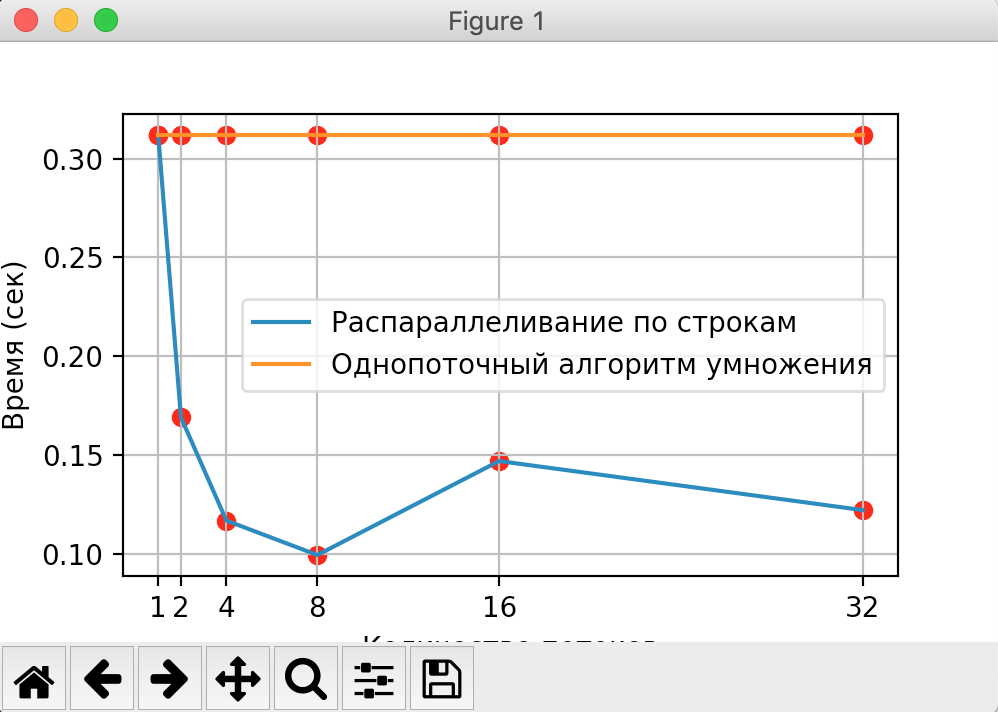
\includegraphics[scale=0.6]{pics/Parallel1.png}
		
			Рис 4.1: Сравнение времени выполнения алгоритмов
\end{center}

В качестве примера в таблице 4.1 представлены временные характеристики однопоточной и многопоточной реализаций стандартного алгоритма умножения матриц при обходе по строкам.

\begin{center}
	\centering
	\caption{Таблица 4.1: Время выполнения однопоточной и многопоточной реализаций стандартного алгоритма умножения матриц}
	\begin{tabular}{|c c|}
		\hline
		Количество потоков & Время  (сек.) \\ [0.5ex] 
 		\hline\hline
		1 & 0.3119\\
 		\hline
 		2 & 0.1691\\
 		\hline
 		4 & 0.1169\\
 		\hline
		8 & 0.0995\\
		\hline
		16 & 0.147\\
		\hline
		32 & 0.1222\\
		\hline
		\end{tabular}
\end{center} 

Как видно из рисунка 4.1 и таблицы 4.1, наибольшая скорость выполнения стандартного алгоритма произведения матриц достигается при параллельной реализации и количестве потоков, равном 8. По сравнению с однопоточной реализацией выигрыш по временной эффективности получается приблизительно в 3 раза. Далее при увеличении числа потоков время выполнения увеличивается, что объясняется очередью потоков (ситуация, когда задач больше, чем потоков)
Рассмотрим временные характеристики алгоритма при фиксированном числе потоков (8) и наборе матриц размерностью [32x1000] x [1000x1000], [64x1000] x [1000x1000], ..., [Nx1000] x [1000x1000], где N = 32*6, (рисунок 4.2).

\begin{center}
		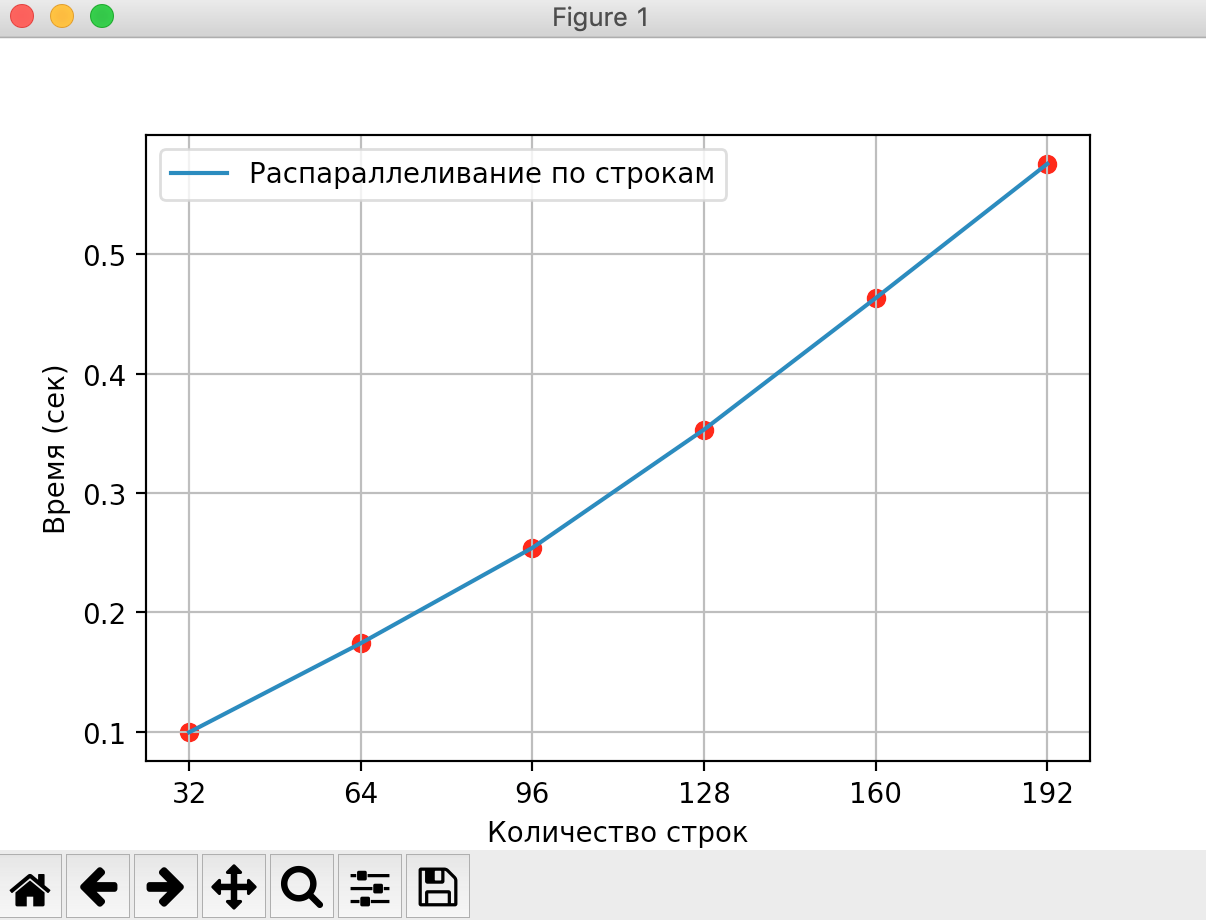
\includegraphics[scale=0.6]{pics/Parallel2.png}
		
			Рис 4.2: Сравнение времени выполнения при разном количестве строк результирующей матрицы и числе потоков, равном 8
\end{center}

Из рисунка 4.2 видно, что время выполнения распараллеленного алгоритма в зависимости от пропорционально увеличивающегося количества обрабатываемых потоками строк растет приблизительной линейно.

\newpage
\section{Результат замеров времени выполнения последовательной и параллельной реализаций стандартного алгоритма умножения матриц при обходе по столбцам} 

Ввиду высокой скорости выполнения вычислений при умножении матриц небольших размеров, для наглядности результатов данного эксперимента возьмем размерность первой матрицы равной [1000x1000], а второй - [1000x32]. При обходе по столбцам количество столбцов результирующей матрицы делится на равные части, которые затем обрабатываются асинхронно и одновременно, каждая одним рабочим потоком. Главный поток запускает рабочие потоки. Эксперимент был проведен со следующим набором потоков: 1, 2, 4, 8, 16, 32. 32 = 4 * 8, где 8 - это количество ядер использовавшейся ЭВМ.

На рисунке 4.3 показана работа однопоточной и многопоточной реализациий стандартного алгоритма умножения матриц при обходе по столбцам.

\begin{center}
		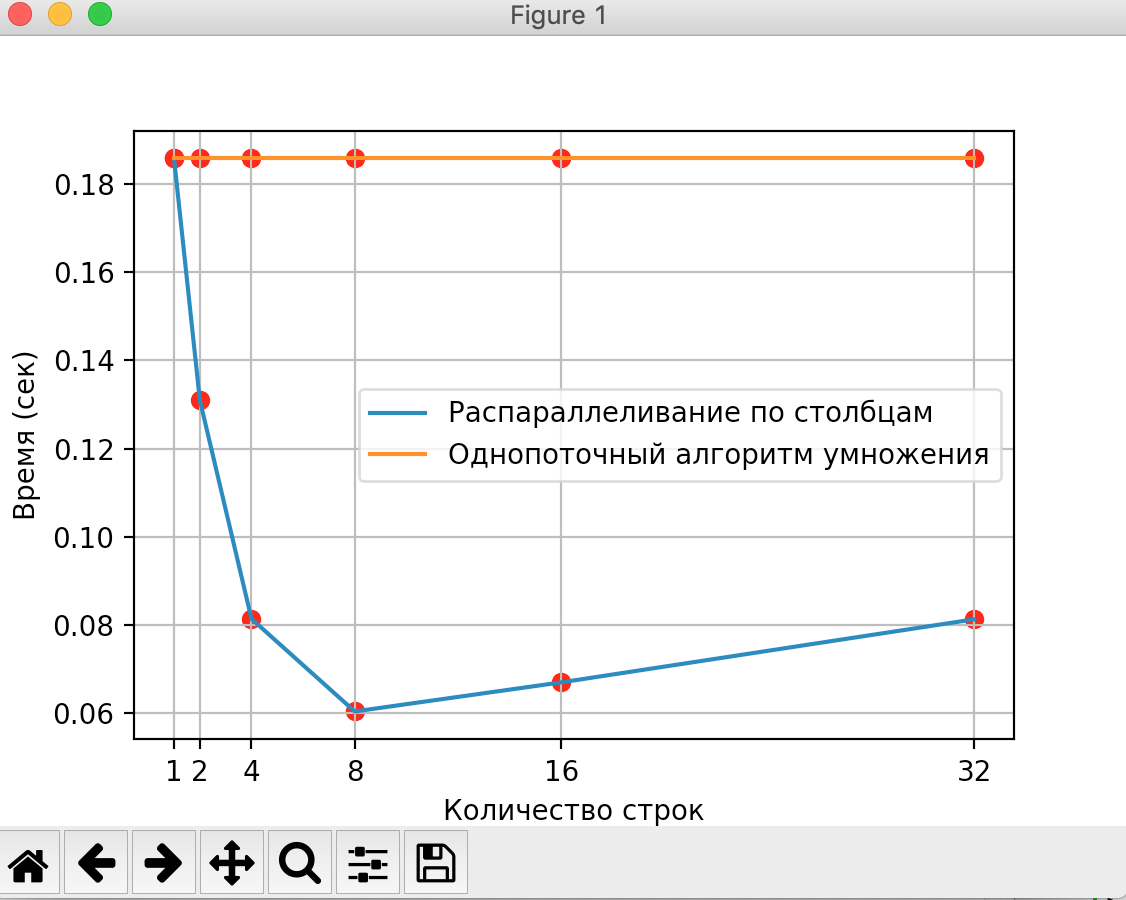
\includegraphics[scale=0.6]{pics/Parallel3.png}
		
			Рис 4.3: Сравнение времени выполнения алгоритмов
\end{center}

В качестве примера в таблице 4.2 представлены временные характеристики однопоточной и многопоточной реализаций стандартного алгоритма умножения матриц при обходе по столбцам.

\begin{center}
	\centering
	\caption{Таблица 4.2: Время выполнения однопоточной и многопоточной реализаций стандартного алгоритма умножения матриц}
	\begin{tabular}{|c c|}
		\hline
		Количество потоков & Время  (сек.) \\ [0.5ex] 
 		\hline\hline
		1 & 0.1858\\
 		\hline
 		2 & 0.131\\
 		\hline
 		4 & 0.0814\\
 		\hline
		8 & 0.0604\\
		\hline
		16 & 0.067\\
		\hline
		32 & 0.0813\\
		\hline
		\end{tabular}
\end{center} 

Как видно из рисунка 4.3 и таблицы 4.2, наибольшая скорость выполнения стандартного алгоритма произведения матриц достигается при параллельной реализации и количестве потоков, равном 8. По сравнению с однопоточной реализацией выигрыш по временной эффективности также получается приблизительно в 3 раза. При увеличении числа потоков вновь возникает очередь к процессору, и, следовательно, производительность снижается.
Рассмотрим временные характеристики алгоритма при фиксированном числе потоков (8) и наборе матриц размерностью [1000x1000] x [1000x32], [1000x1000] x [1000x64], ..., [Mx1000] x [1000x1000], где M = 32 * 6, (рисунок 4.4).

\begin{center}
		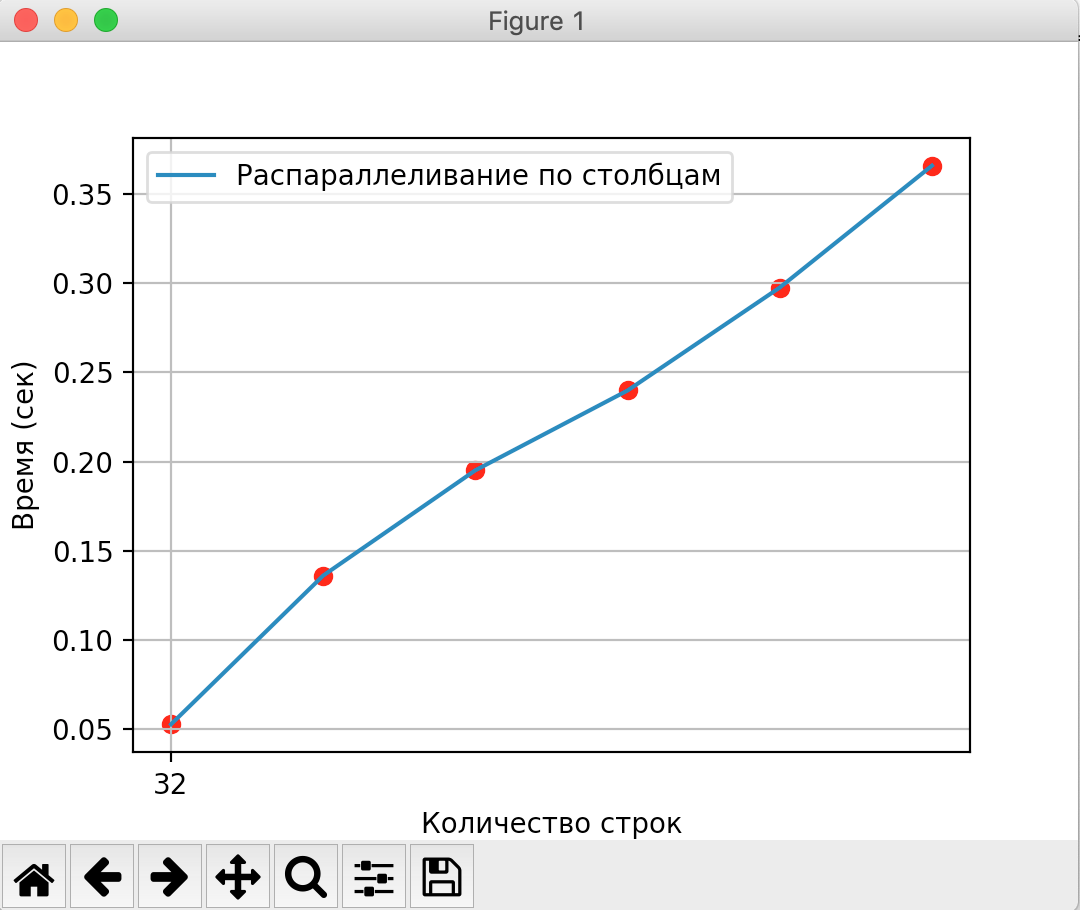
\includegraphics[scale=0.6]{pics/Parallel4.png}
		
			Рис 4.4: Сравнение времени выполнения при разном количестве столбцов результирующей матрицы и числе потоков, равном 8
\end{center}

Из рисунка 4.4 видно, что время выполнения распараллеленного алгоритма в зависимости от пропорционально увеличивающегося количества обрабатываемых потоками строк растет приблизительной линейно.

\section{Вывод}

В ходе эксперимента было установлено, что максимальной эффективности по времени стандартный алгоритм умножения матриц достигает при параллельной реализации с использованием 8 потоков, следовательно, при задействовании всех логических ядер ЭВМ, участвовавшей в эксперименте.


\chapter*{Заключение}
\addcontentsline{toc}{chapter}{Заключение}
В ходе лабораторной работы были реализованы и проанализированы последовательная и параллельная реализации стандартного алгоритма умножения матриц. 

В рамках выполнения работы решены следующие задачи.

\begin{enumerate}
\item Изучены основы многопоточного программирования.
\item  Придуманы два варианта многопоточной реализации стандартного алгоритма умножения матриц: обход по строкам и обход по столбцам.
\item Программно реализован стандартный алгоритм умножения матриц в однопоточном режиме.
\item Сделан сравнительный анализ по затрачиваемым ресурсам (времени) компьютера на реализацию каждого рассмотренного алгоритма.
\end{enumerate}

%\bibliographystyle{gost780u}
%\bibliography{books}


\addcontentsline{toc}{chapter}{Список литературы}
\begin{thebibliography}{3}
	\bibitem{Vs}
	Visual Studio [Электронный ресурс], режим доступа:https://visualstudio.microsoft.com/ru/ (дата обращения: 01.10.2020)
	\bibitem{Stopwatch}
	Thread.Join Метод [Электронный ресурс], режим доступа:https://docs.microsoft.com/ru-ru/dotnet/api/system.threading.thread.join?view=netcore-3.1 (дата обращения: 01.10.2020)
	\bibitem{C}
	Документация по C\# [Электронный ресурс], режим доступа:https://docs.microsoft.com/ru-ru/dotnet/csharp/ (дата обращения: 02.10.2020)
	\bibitem{MicrosoftPar}
	Академия Microsoft: Основы параллельного программирования с использованием Visual Studio [Электронный ресурс], - режим доступа: https://intuit.ru/studies/courses/4807/1055/lecture/16369 (дата обращения: 02.10.2020)
	\bibitem{Rand}
	Random Класс [Электронный ресурс], режим доступа:https://docs.microsoft.com/ru-ru/dotnet/api/system.random?view=netcore-3.1 (дата обращения: 01.10.2020)
\end{thebibliography}


\end{document}